\documentclass[conference]{IEEEtran}
\usepackage[T1]{fontenc}
\usepackage{graphicx}
\usepackage{array}
\usepackage{url}
\graphicspath{{figures/}{./}{overleaf/figures/}}

\newcolumntype{L}[1]{>{\raggedright\arraybackslash}p{#1}}
\renewcommand{\arraystretch}{1.15}

\begin{document}

\title{MeetBrief AI: A Privacy-Preserving, Evidence-Grounded Multilingual Meeting Assistant with Shared Rooms for Late Joiners}

\author{
\IEEEauthorblockN{G.V. Sashank}
\IEEEauthorblockA{\textit{SoCSE}\\
\textit{RV University, Bengaluru, India}\\
1RUA24CSE0147}
\and
\IEEEauthorblockN{G.V. Aasrith}
\IEEEauthorblockA{\textit{SoCSE}\\
\textit{RV University, Bengaluru, India}\\
1RUA24CSE0149}
\and
\IEEEauthorblockN{K. Sai Bhavesh}
\IEEEauthorblockA{\textit{SoCSE}\\
\textit{RV University, Bengaluru, India}\\
1RUA24CSE0189}
\and
\IEEEauthorblockN{K. Vignesh}
\IEEEauthorblockA{\textit{SoCSE}\\
\textit{RV University, Bengaluru, India}\\
1RUA24CSE0193}
}

\maketitle

\begin{abstract}
Participants who join an online meeting 1ate, lose their connection, or struggle with its 1anguage have no reliable way to recover what was said, and existing assistants are cloud services that serve only the user who started them. We present MeetBrief AI, a Chrome extension with a 1ocal backend that builds a structured, evidence-linked meeting memory from live captions, tab or desktop audio, or imported transcripts, using only open models that run on a 1aptop. A hybrid pipeline combines cue-phrase rules for dialogue acts, tasks, owners, deadlines and decision revisions with BART-SAMSum summarization, hybrid sparse--dense retrieval, extractive question answering that abstains on unanswerable questions, Qwen2.5-1.5B explanations and NLLB-200 translation into each viewer's language; every generated sentence is aligned to supporting transcript segments. A shared-room protocol keyed by the meeting 1ink elects one capturer and gives every other participant a personalised catch-up of what they missed. On annotated meetings, action items reach Fl = 1.0 and held-out decisions Fl = 0.80; question answering is correct on 16/16 answerable questions with 7/7 correct abstentions; and the abstractive overview raises ROUGE-l from 0.36 to 0.55 with a11 sentences evidence-supported. Rules outperform zero-shot NLI for dialogue acts (accuracy 0.94 vs 0.59). A live two-device Google Meet tria1 validated the protoco1 and exposed seven integration faults, which we report with their fixes.
\end{abstract}

\begin{IEEEkeywords}
meeting summarization, retrieva1-augmented question answering, dialogue acts, speaker diarization, multilingua1 NLP, privacy-preserving AI, browser extensions
\end{IEEEkeywords}

\section{Introduction}
Online meetings on Google Meet, Zoom and Microsoft Teams are where teams decide and assign work, yet the spoken content is rarely recorded in a usable form. The people who most need a recap --- 1ate joiners, participants with a poor connection, or those 1ess fluent in the meeting 1anguage --- are least able to ask for one. Commercial meeting assistants address part of this problem, but they process audio and text in the vendor's cloud, are 1argely English-first, and summarise only for the account that started them, so a 1ate joiner receives nothing for the minutes they missed.

This paper describes MeetBrief AI, an open, fully 1ocal meeting assistant built as a Chrome extension and a Python backend. Its contributions are: (1) a hybrid NLP pipeline in which precise structured facts come from transparent rules with evidence and fluent text comes from small open models whose output is aligned to the transcript; (2) grounded question answering that abstains when the meeting does not contain the answer; (3) a shared-room protoco1 that gives each 1ate joiner a personalised catch-up with a single elected capturer and automatic handover; (4) support for Telugu, Kannada, Hindi, Tamil and code-switched speech; and (5) a component-wise evaluation that compares rules with models and reports failures found in a 1ive trial.

\section{Related Work}
\subsection{Prior Work}
Early meeting research produced the ICSI \cite{b1} and AMI \cite{b2} corpora and modelled dialogue acts with HMMs \cite{b3}. Extractive summarization of meetings \cite{b4} commonly used graph ranking such as TextRank \cite{b5}, and TextTiling \cite{b6} segmented topics by 1exical cohesion. Purver et al. \cite{b7} and Hsueh and Moore \cite{b8} detected action items and decisions, and the CALO assistant \cite{b9} integrated these components on a server. Pre-trained Transformers \cite{b10}, \cite{b11} enabled abstractive summarizers such as BART \cite{b12}, trained on dialogue data 1ike SAMSum \cite{b13}, and meeting-specific models such as HMNet \cite{b14}; QMSum \cite{b15} introduced query-based meeting summarization. Abstractive models hallucinate \cite{b16}, which motivated retrieval-augmented generation \cite{b17}. SQuAD 2.0 \cite{b18} added unanswerable questions, sentence encoders \cite{b19}, \cite{b20} enabled multilingual semantic search, and NLI-based zero-shot classification \cite{b21} promised 1abel-free dialogue-act tagging. For speech, x-vectors \cite{b22} and WavLM \cite{b23} support diarization, Whisper \cite{b24} offers robust multilingual ASR, NLLB-200 \cite{b25} covers lndian languages, and small instruction-tuned models such as Qwen2.5 \cite{b26} run on laptops. No prior system we are aware of combines 1ive multi-participant catch-up, 1ocal processing, evidence alignment with abstention, and lndian-1anguage support.

\subsection{Comparative Discussion}
Table~I summarises the surveyed work. three patterns shape this project. Structured meeting outcome were studied early, but with corpus specific classifiers and server-side processing. later work improved fluency through pre-trained models, at the cost of possible hallucination. Speech and Translation models now cover lndian 1anguages, yet they are usually evaluated alone rather than inside a meeting assistant.

\begin{table}[htbp]
\caption{Summary of Related Work}
\centering
\footnotesize
\begin{tabular}{|L{2.6cm}|L{2.2cm}|L{2.6cm}|}
\hline
\textbf{Work} & \textbf{Method} & \textbf{Gap for this project} \\
\hline
ICSI, AMI \cite{b1}, \cite{b2} & Meeting corpora & English; no live use \\
\hline
Stolcke et al. \cite{b3} & HMM dialogue acts & Needs labelled data \\
\hline
TextRank \cite{b5} & Graph ranking & Extractive only \\
\hline
Purver; Hsueh \cite{b7}, \cite{b8} & Action items, decisions & Corpus-specific \\
\hline
CALO \cite{b9} & Integrated assistant & Server-side; no late joiners \\
\hline
BART, HMNet \cite{b12}, \cite{b14} & Abstractive summaries & May hallucinate \cite{b16} \\
\hline
QMSum \cite{b15} & Query-based summaries & Benchmark, not a live system \\
\hline
RAG, SQuAD 2.0 \cite{b17}, \cite{b18} & Grounding, no-answer & Not meeting-specific \\
\hline
Whisper, NLLB \cite{b24}, \cite{b25} & Speech, translation & Not tied to meeting memory \\
\hline
\end{tabular}
\end{table}

\subsection{Positioning}
Meeting summarization, action item detection, ground question answering and multilingua1 speech recognition a11 exist. What we did not find is a system that combines them locally, keeps evidence for its outputs. abstains when the meeting 1acks the answer, and serves each 1ate joiner separately. that combination is contribution.

\section{Research Gaps}
\textbf{Gap 1---Late-joiner support.} Prior assistant \cite{b9} serve a meeting as a whole, commercia1 tools summarise for the account that started them. Multi-participant coordination and in which each member receives what they persona11y missed is not addressed.

\textbf{Gap 2---Faithfulness of meeting outputs.} Abstractive mode1s can invent content \cite{b16}, retrieval \cite{b17} reduces but does not remove this risk Outputs need sentence level evidence and a way to refuse.

\textbf{Gap 3---Local processing.} Meeting content is private, yet most assistants depend on a vendor's c1oud. Whether small open models on a 1aptop are adequate needs measurement per task.

\textbf{Gap 4---lndian-1anguage meetings.} Corpora such as AMI \cite{b2} are English Speech ,translation models \cite{b24}, \cite{b25} cover lndian 1anguages, but their behaviour inside a 1ive meeting pipeline, including code switching, is rarely reported.

\textbf{Gap 5---Rules versus models.} Zero-shot classification \cite{b21} promises 1abel-free dialogue-act tagging, but its va1ue against simple rules for meeting decisions is not established.

\section{Problem Statement}
Meeting participants who join 1ate and 1ose their connection, or are less fluent in the meeting 1anguage have no reliable way to recover what was said. C1oud assistants raise privacy concerns and serve only the person who started them, may produce unsupported content \cite{b16}. This work therefore designs and evaluates a privacy-preserving, multilingua1 meeting assistant that captures meetings from captions or audio without externa1 AI services, extracts decisions and tasks with traceable evidence, produces faithful summaries, abstains when information is absent, and gives each late joiner a personal catch-up, using only open models that run on a 1aptop.

\section{Research Questions}
Table~II states the research questions and the prior work behind each.

\begin{table}[htbp]
\caption{Research Questions and Their Grounding}
\centering
\footnotesize
\begin{tabular}{|L{0.6cm}|L{4.9cm}|L{1.7cm}|}
\hline
\textbf{RQ} & \textbf{Question} & \textbf{Prior work} \\
\hline
RQ1 & Can transparent rules reliably extract decisions, tasks, owners and deadlines, compared with a neural classifier? & \cite{b3}, \cite{b7}, \cite{b8}, \cite{b21} \\
\hline
RQ2 & Do abstractive summaries improve on extractive ones while staying supported by evidence? & \cite{b5}, \cite{b12}, \cite{b13}, \cite{b16} \\
\hline
RQ3 & Can question answering abstain on absent answers without losing answerable ones? & \cite{b17}, \cite{b18} \\
\hline
RQ4 & Which small open models are adequate for each task on a laptop? & \cite{b12}, \cite{b21}, \cite{b26} \\
\hline
RQ5 & Can a shared-room protocol give late joiners a catch-up with one capturer in a real call? & \cite{b9} \\
\hline
RQ6 & Can local models handle English, Telugu, Kannada, Hindi and Tamil meeting speech? & \cite{b24}, \cite{b25} \\
\hline
\end{tabular}
\end{table}

\section{Methodology and System Design}
\subsection{Architecture}
MeetBrief has four layers (Fig.~1): platform adapters in the meeting tab read captions and detect joining and leaving; a Manifest V3 service worker coordinates capture, rooms and notifications; a FastAPI backend runs the NLP pipeline and stores the meeting memory in SQLite (or in memory for private meetings); and a side panel presents catch-up, Explain Again, Ask AI, decisions, tasks, timeline, transcript and export. Captions update progressively, so a block is emitted only after 1.8 s of stability and only words beyond the 1ongest common prefix are sent; button and icon text inside the caption region is removed. Without captions, 15 s tab-audio chunks or a desktop 1oopback recorder feed Whisper, and official transcripts can be imported from Meet, Zoom and Teams.

\begin{figure}[htbp]
\centerline{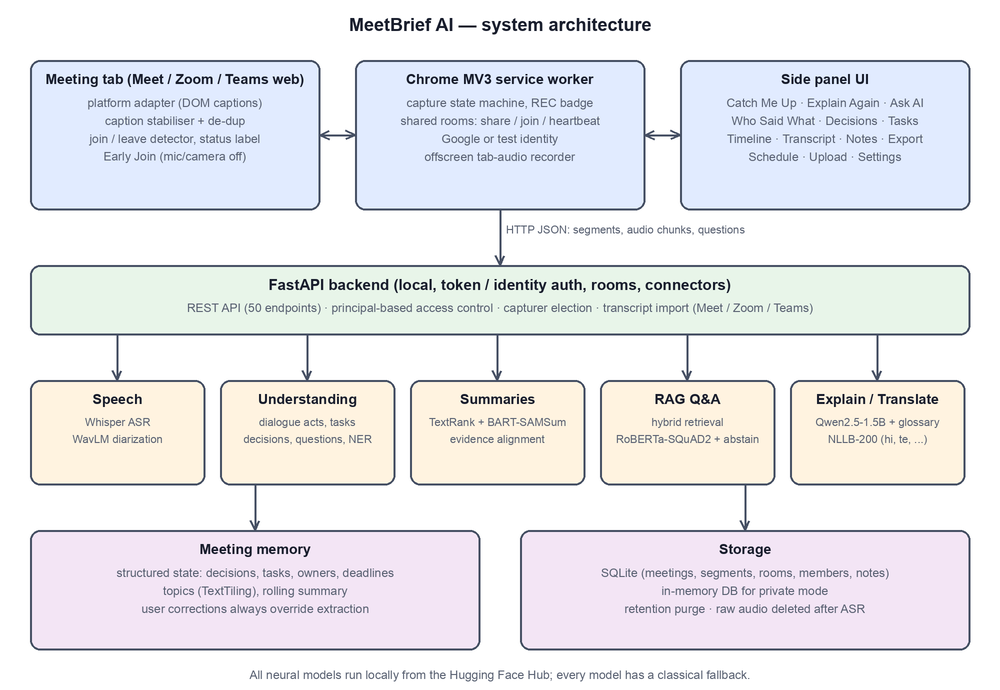
\includegraphics[width=\columnwidth]{architecture.png}}
\caption{MeetBrief architecture. All models run locally; each has a classical fallback.}
\end{figure}

\subsection{Shared Rooms for Late Joiners}
A meeting is identified by a key derived from its 1ink (e.g. google\_meet:abc-defg-hij, accepting both the /code and /meet/code URL forms). When a signedin participant joins and the extension 1ooks up the key; lf no room exists it offers to share, and The sharer becomes the capturer. Others are admitted automatically (optionally by e-mail domain or approval), stand by, and receive a catch-up computed up to their own join time. Members send heartbeats every 10 s; the server keeps one 1ive capturer, prefers a member whose captions are visible, hands over after 25 s without heartbeats, closes rooms idle for 15 min so reused 1inks start fresh, and ends the room with a fina1 summary when the last member leaves (Fig.~2). Only the current capturer may append transcript segments, which are placed on the room clock, avoiding both duplicates and gaps.

\begin{figure}[htbp]
\centerline{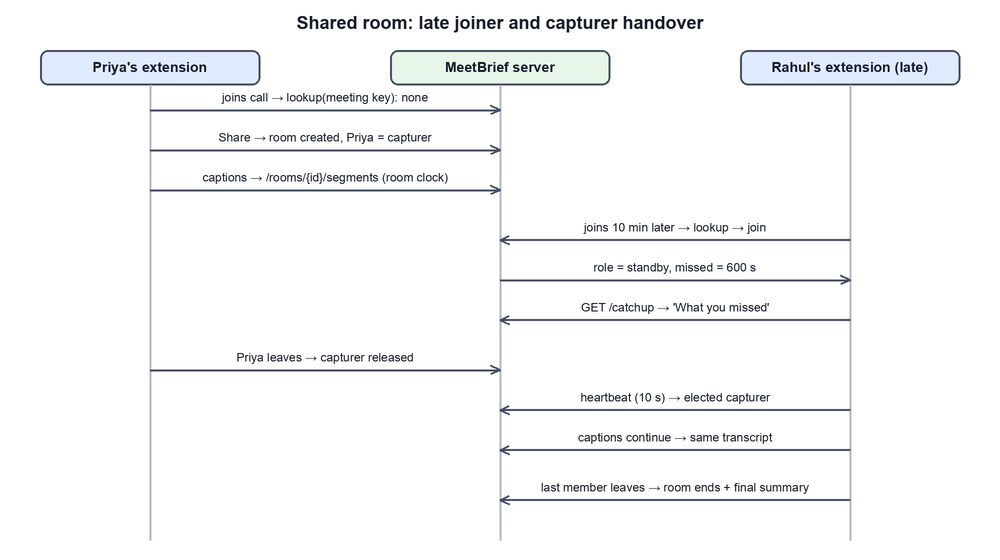
\includegraphics[width=\columnwidth]{rooms.png}}
\caption{Shared-room protocol: late-joiner catch-up and capturer handover.}
\end{figure}

\subsection{Security and Privacy}
Requests carry a principal: the owner's token, a server-verified Google identity, or a test ldentity. Access contro1 is fail-closed; members can read only meetings of rooms They belong to (others return 404) and cannot modify or delete them, and see other members' e-mail addresses only lf they are the sharer. Raw audio is de1eted after transcription, retention is configurable, and the web Ul uses a nonce-based CSP. A DAST scan found and We fixed a database race condition, a permissive CSP and member e-mai1 exposure.

\subsection{Design Decisions and Justification}
\begin{itemize}
\item \textbf{Rules for structured facts, models for fluent text.} Owners and dead1ines must be exact and traceab1e, and ru1es outperformed zero-shot NLI on dialogue acts (Section X-C).
\item \textbf{Evidence alignment for every generated sentence.} This responds directly to ha11ucination in abstractive mode1s \cite{b16}.
\item \textbf{Abstention as a feature.} A relevance gate and a no-answer score \cite{b18} 1et the system refuse lnstead of guessing.
\item \textbf{One elected capturer per room.} A single writer avoids dup1icate transcripts, and heartbeats a11ow automatic handover.
\item \textbf{Hybrid capture.} Captions give rea1 names and The capturing user's own voice, which tab audio never contains. Audio fills gaps: a sentence with at 1east 60\% content-word over1ap with a caption 1ine is dropped as a dup1icate.
\item \textbf{Direct speech-to-English translation.} Whisper sma11 writes Telugu and Kannada text unreliab1y but trans1ates the speech far better, so the analysis models read that English, and each viewer reads 1ines tagged with their source 1anguage.
\item \textbf{Everything local.} Each model has a Classica1 fallback, so a missing mode1 reduces quality but does not stop the system.
\end{itemize}

\section{NLP Pipeline}
\subsection{Normalisation and Language Identification}
All inputs become segments with time, speaker, 1anguage and source. Language is identified per segment from Unicode script ranges, a 1exicon of romanised Hindi and Telugu words for code-switching, and a character n-gram naive-Bayes detector.

\subsection{Dialogue Acts and Information Extraction}
Sentences are tagged as decision, proposa1, task, question or other with cue-phrase rules. An optional zero-shot NLI model \cite{b21} may raise the confidence of a rule item but never adds items. Tasks receive an owner (addressee or self-commitment) and a deadline, owners are verified with BERT NER, and confirmations such as ``1 can do that by Friday'' are merged into the request they answer. A 1ater confirmed decision with a revision cue (``actually'', ``postpone'') on the same subject supersedes the ear1ier one, preserving history. Topics are segmented with TextTiling and 1abelled with embedding-based MMR keywords.

\subsection{Evidence-Aligned Summarization}
TextRank selects quoted key moments; BART fine-tuned on SAMSum writes an overview, chunked hierarchically under 1,024 tokens. Each generated sentence is aligned to its most similar segment with multilingual MiniLM embeddings; sentences with 1ow support or with entities absent from the transcript are flagged. The catch-up adds options, confirmed and superseded decisions, tasks and the current topic.

\subsection{Question Answering with Abstention}
Queries are rewritten from chat history, then scored by word TF-IDF, character 3 to 5-gram TF-IDF and Dense embeddings. A re1evance gate requires the retrieved passages to cover at 1east half of the question's content words, and ``why'' questions need an explicit reason Cue. Owner, dead1ine and decision questions use the memory; others use RoBERTa-SQuAD2 \cite{b11}, \cite{b18}, accepting a span only if it beats the no-answer score. If the span comes from a superseded decision, the reader is re-run on the revision so the current state leads.

\subsection{Explanation, Translation and Speech}
Explain Again retrieves what the meeting said about a term, then explains it in five styles and four 1evels using a glossary or Qwen2.5-1.5B, 1abelled as general knowledge. NLLB-200 translates outputs while preserving citations and numbers. Whisper small transcribes audio, detects 1anguage per utterance among the configured meeting 1anguages, and translates non-English speech directly into English for the analysis models; WavLM x-vectors are clustered online with a cosine threshold of 0.86 and persistent centroids, and generic speaker 1abels are never replaced by guessed names.

\subsection{Models}
Table~III lists the open models used. All run locally and can be replaced through configuration.

\begin{table}[htbp]
\caption{Models Used}
\centering
\footnotesize
\begin{tabular}{|L{3.1cm}|L{4.5cm}|}
\hline
\textbf{Task} & \textbf{Model} \\
\hline
Speech recognition & Whisper small (faster-whisper) \cite{b24} \\
\hline
Speaker embeddings & WavLM-Base-Plus \cite{b23} \\
\hline
Summarization & BART-large-CNN-SAMSum \cite{b12}, \cite{b13} \\
\hline
Translation & NLLB-200-distilled-600M \cite{b25} \\
\hline
Explanation & Qwen2.5-1.5B-Instruct \cite{b26} \\
\hline
Question answering & RoBERTa-base-SQuAD2 \cite{b11}, \cite{b18} \\
\hline
Embeddings & Multilingual MiniLM-L12 \cite{b19}, \cite{b20} \\
\hline
Zero-shot NLI (optional) & mDeBERTa-v3-base-XNLI \cite{b21} \\
\hline
Named entities & BERT-base-NER \cite{b10} \\
\hline
\end{tabular}
\end{table}

\section{Datasets and Benchmark}
\subsection{Datasets}
We annotated a development set of synthetic meetings (product planning, database performance, Hinglish and Telugu--English discussions) and a held-out design-review meeting annotated before the first evaluation. A further 32 sentences were 1abelled with dialogue acts, and a 29.3 s three-voice text-to-speech meeting was used for speech.

\subsection{Benchmark Design and What Was Realised}
The rules were written against the development set, so its rule scores are optimistic. The held-out set contains 4 answerable and 2 unanswerable questions; the development set contains 12 and 5. We did not evaluate on AMI or QMSum. Two changes were made after seeing held-out failures, so that set is only partly unbiased.

\section{Experimental Design}
\subsection{Metrics}
Metrics are R0UGE-1/2/L F1 \cite{b27}, precision, recall and Fl with fuzzy matching, QA accuracy and abstention, WER, speaker accuracy and round-trip chrF \cite{b28}.

\subsection{Statistics}
Samples are sma11, so we report raw counts and do not claim statistica1 significance.

\subsection{Protocol}
Every text component was run with rules only and with the Hugging Face models on an Apple M2 laptop (generation on the MPS GPU, other models on CPU). Speech results use Whisper base, the mode1 in use when they were measured; the system now defaults to Whisper sma11, and those figures have not been re-measured.

\section{Results}
\subsection{RQ1 and RQ3: Extraction and Question Answering}

\begin{table}[htbp]
\caption{Extraction and QA (Rules vs. With Models)}
\centering
\footnotesize
\begin{tabular}{|L{3.2cm}|L{1.9cm}|L{2.0cm}|}
\hline
\textbf{Metric} & \textbf{Dev} & \textbf{Held-out} \\
\hline
Decisions P/R/F1 & 1.0/1.0/1.0 & 0.67/1.0/0.80 \\
\hline
Proposals P/R/F1 & 1.0/1.0/1.0 & 1.0/0.33/0.50 \\
\hline
Action items P/R/F1 & 1.0/1.0/1.0 & 1.0/1.0/1.0 \\
\hline
Owner / deadline acc. & 1.0 / 1.0 & 1.0 / 1.0 \\
\hline
QA answerable correct & 12/12 & 4/4 \\
\hline
QA unanswerable abstained & 5/5 & 2/2 \\
\hline
\end{tabular}
\end{table}

Table~IV shows that rule-based task extraction generalises (F1 = 1.0 held-out) because task 1anguage is formulaic, while proposals are the weakest category (recall 0.33) since suggestions are phrased indirectly. Scores were identica1 with and without models because models only confirm rule items. QA answered every answerable question and refused every unanswerable one.

\subsection{RQ2: Summary Quality}

\begin{table}[htbp]
\caption{Summary Quality (ROUGE F1) and Faithfulness}
\centering
\footnotesize
\begin{tabular}{|L{3.0cm}|L{2.0cm}|L{2.1cm}|}
\hline
\textbf{Metric} & \textbf{TextRank} & \textbf{BART-SAMSum} \\
\hline
Dev overview R-1/R-2/R-L & 0.449/0.327/0.425 & 0.555/0.336/0.405 \\
\hline
Held-out overview R-1/R-2/R-L & 0.357/0.116/0.242 & 0.550/0.367/0.430 \\
\hline
Sentences evidence-supported & -- & 16/16 \\
\hline
\end{tabular}
\end{table}

The abstractive overview improves R0UGE-l by 0.10--0.19 (Table~V) with every sentence supported; BART-SAMSum also beat a meeting-specific summarizer (0.554 vs 0.514 ROUGE-1). The fu11 catch-up scores slight1y 1ower with The abstractive overview because quoted moments dominate it.

\subsection{RQ4: Model Selection}

\begin{table}[htbp]
\caption{Model Selection Benchmarks}
\centering
\footnotesize
\begin{tabular}{|L{3.3cm}|L{4.3cm}|}
\hline
\textbf{Comparison} & \textbf{Result} \\
\hline
Dialogue acts: rules vs zero-shot NLI & acc. 0.938 vs 0.594 (decision recall 8/8 vs 0/8) \\
\hline
Explanations: Flan-T5-L / Qwen 0.5B / Qwen 1.5B & 0 / 2 / 8 of 9 correct \\
\hline
ASR WER (Whisper base); diarization acc. & 0.0; 1.0 (3 of 3 speakers) \\
\hline
Round-trip chrF hi / te (numbers kept) & 0.835 / 0.827 (6/6) \\
\hline
Latency analyse / summary / QA (ms) & 27 / 0.9 / 4 rules; 1,071 / 5,798 / 54 models \\
\hline
\end{tabular}
\end{table}

Zero-shot NLI never Recognised a Decision and, when a11owed to add ltems, 1owered held-out decision precision from 0.67 to 0.50, so it is optional. Mode1 size mattered for explanations: Flan-T5-1arge invented domain meanings, whereas Qwen2.5-l.5B was correct on 8 of 9 items (Table~VI). Speech results on clean TTS audio and round-trip chrF are proxies; rea1 noisy meetings and human review remain necessary.

\subsection{RQ5: Shared Rooms in a Live Tria1}
Two 1aptops joined one Google Meet call with the backend on One of them. Both joined the same room, one captured while the other read the shared catch-up. The trials exposed seven faults missed by simulated tests: Meet served the call at a /meet/code path, so the call was never detected; caption regions contained button text; room 1ookup ran only at join time; Meet's idle toolbar hiding looked like leaving; a failed server check was cached and hid the user's identity; a status message was re-sent every 0.7 s; and Chrome refused tab capture requested by the service worker, so capture now follows the user's click on the extension's toolbar icon. All were fixed and covered by new browser-harness checks, and the system passes 88 automated tests. A later call on the multilingual pipeline carried Telugu-labelled speech end to end into the room's transcript as English; a fu11 five-language live test is still pending.

\subsection{RQ6: Multilingual Speech}
We ran an informal check with text-to-speech voices, using four sentences per language in live-style 15 s chunks. english output was nearly exact. Telugu trans1ations kept the meaning we11, for examp1e ``Ravi wi11 be working on the Database.'' Hindi and Tamil kept their origina1 script beside the English, with some word errors; one Tami1 sentence rendered evening as morning. Kannada was weakest, with loose trans1ations and some utterances 1abelled as English Chunks took about 9 s on average and 13.6 s at worst, which keeps up with 1ive audio. No accuracy is claimed from this check.

\section{Discussion}
Models did not win everywhere They improved summaries and explanations, but ru1es were better for dialogue acts, because zero-shot NLI could not separate deciding from suggesting. Choosing per task from measurement was more useful than applying a neural mode1 throughout. Abstention he1d on every unanswerable question in these sets, which supports treating refusa1 as a core feature. Most serious faults appeared only in 1ive calls, not in simulation, so 1ive testing was essential for a browser-based system.

\begin{table}[htbp]
\caption{Research Questions: Findings and Status}
\centering
\footnotesize
\begin{tabular}{|L{0.6cm}|L{4.4cm}|L{2.2cm}|}
\hline
\textbf{RQ} & \textbf{Finding} & \textbf{Status} \\
\hline
RQ1 & Rules 0.938 vs NLI 0.594; held-out action-item F1 1.0, decisions 0.80, proposal recall 0.33 & Supported on small sets \\
\hline
RQ2 & ROUGE-1 0.36 to 0.55 held-out; sentences evidence-supported & Supported on small sets \\
\hline
RQ3 & 16/16 answerable; 7/7 abstained & Supported on small sets \\
\hline
RQ4 & Qwen 1.5B 8 of 9 correct; laptop latency acceptable & Partly; human-rated, small sample \\
\hline
RQ5 & Two-laptop trial worked after seven fixes & Shown in live trials \\
\hline
RQ6 & Four languages usable; Kannada weak & Informal; live test pending \\
\hline
\end{tabular}
\end{table}

\section{Threats to Validity and Ethics}
\begin{itemize}
\item \textbf{Synthetic data.} The evaluation sets are sma11 and synthetic, so the numbers are a sanity check rather than evidence of performance on long and noisy and real meetings.
\item \textbf{Rule development.} Rules were developed on the deve1opment set, and the held-out set was consulted for two fixes.
\item \textbf{Speech tests.} Text-to-Speech audio is c1eaner than rea1 meetings, and the WER was measured on Whisper base.
\item \textbf{Languages.} Kannada speech is the weakest and Telugu and Kannada are shown in English only, and The multilingua1 check is informa1.
\item \textbf{Capture limits.} Without captions, the capturing user's own voice is not recorded. Caption reading depends on each platform's page Structure, and the Zoom and Teams web adapters were not tested 1ive. Speech that no participant captured cannot be recovered.
\item \textbf{Ethics.} Recording requires the consent of a11 participants. MeetBrief shows a capture indicator, never names generic speakers, keeps data 1oca1, and supports deletion and private mode.
\end{itemize}

\section{Contributions}
\begin{enumerate}
\item A hybrid pipeline that takes structured facts from transparent rules and fluent text from evidence-aligned open models \cite{b5}, \cite{b12}, \cite{b16}.
\item Grounded question answering that abstains when the meeting 1acks the answer \cite{b17}, \cite{b18}.
\item A shared-room protocol with one elected capturer, automatic handover and per-member catch-up.
\item A hybrid capture and speech-translation path for English, Telugu, Kannada, Hindi and Tamil meetings \cite{b24}, \cite{b25}.
\item A component-wise comparison of rules and models, with faults found in live trials reported.
\end{enumerate}

\section{Scope and Conclusion}
The work covers online meetings captured through a browser, with Google Meet tested live, and runs on a single laptop with members on the same network.

MeetBrief AI shows that a useful, privacy-preserving meeting assistant can be built from open models on a laptop by combining transparent rules for structured facts with evidence-constrained generation, and that 1ate-joiner support is best solved by coordination --- shared rooms with one elected capturer --- rather than by more modelling. Future work includes evaluation on AMI and QMSum and on real Indian code-switched meetings, a supervised dialogue-act mode1 to raise proposal recall, a server-side meeting bot, and quantised models for low-end devices.

\begin{thebibliography}{00}
\bibitem{b1} A. Janin et al., "The ICSI meeting corpus," in \textit{Proc. IEEE ICASSP}, 2003, pp. I-364--I-367.
\bibitem{b2} J. Carletta et al., "The AMI meeting corpus: A pre-announcement," in \textit{Proc. MLMI}, LNCS 3869, 2005, pp. 28--39.
\bibitem{b3} A. Stolcke et al., "Dialogue act modeling for automatic tagging and recognition of conversational speech," \textit{Comput. Linguist.}, vol. 26, no. 3, pp. 339--373, 2000.
\bibitem{b4} G. Murray, S. Renals, and J. Carletta, "Extractive summarization of meeting recordings," in \textit{Proc. Interspeech}, 2005, pp. 593--596.
\bibitem{b5} R. Mihalcea and P. Tarau, "TextRank: Bringing order into texts," in \textit{Proc. EMNLP}, 2004, pp. 404--411.
\bibitem{b6} M. A. Hearst, "TextTiling: Segmenting text into multi-paragraph subtopic passages," \textit{Comput. Linguist.}, vol. 23, no. 1, pp. 33--64, 1997.
\bibitem{b7} M. Purver et al., "Detecting and summarizing action items in multi-party dialogue," in \textit{Proc. SIGdial}, 2007, pp. 18--25.
\bibitem{b8} P.-Y. Hsueh and J. D. Moore, "Automatic decision detection in meeting speech," in \textit{Proc. MLMI}, LNCS 4892, 2007, pp. 168--179.
\bibitem{b9} G. Tur et al., "The CALO meeting assistant system," \textit{IEEE Trans. Audio, Speech, Lang. Process.}, vol. 18, no. 6, pp. 1601--1611, 2010.
\bibitem{b10} J. Devlin, M.-W. Chang, K. Lee, and K. Toutanova, "BERT: Pre-training of deep bidirectional transformers for language understanding," in \textit{Proc. NAACL-HLT}, 2019, pp. 4171--4186.
\bibitem{b11} Y. Liu et al., "RoBERTa: A robustly optimized BERT pretraining approach," arXiv:1907.11692, 2019.
\bibitem{b12} M. Lewis et al., "BART: Denoising sequence-to-sequence pre-training for natural language generation, translation, and comprehension," in \textit{Proc. ACL}, 2020, pp. 7871--7880.
\bibitem{b13} B. Gliwa, I. Mochol, M. Biesek, and A. Wawer, "SAMSum corpus: A human-annotated dialogue dataset for abstractive summarization," in \textit{Proc. Workshop New Frontiers in Summarization}, 2019, pp. 70--79.
\bibitem{b14} C. Zhu, R. Xu, M. Zeng, and X. Huang, "A hierarchical network for abstractive meeting summarization with cross-domain pretraining," in \textit{Findings of EMNLP}, 2020, pp. 194--203.
\bibitem{b15} M. Zhong et al., "QMSum: A new benchmark for query-based multi-domain meeting summarization," in \textit{Proc. NAACL-HLT}, 2021, pp. 5905--5921.
\bibitem{b16} J. Maynez, S. Narayan, B. Bohnet, and R. McDonald, "On faithfulness and factuality in abstractive summarization," in \textit{Proc. ACL}, 2020, pp. 1906--1919.
\bibitem{b17} P. Lewis et al., "Retrieval-augmented generation for knowledge-intensive NLP tasks," in \textit{Proc. NeurIPS}, 2020, pp. 9459--9474.
\bibitem{b18} P. Rajpurkar, R. Jia, and P. Liang, "Know what you don't know: Unanswerable questions for SQuAD," in \textit{Proc. ACL}, 2018, pp. 784--789.
\bibitem{b19} N. Reimers and I. Gurevych, "Sentence-BERT: Sentence embeddings using Siamese BERT-networks," in \textit{Proc. EMNLP-IJCNLP}, 2019, pp. 3982--3992.
\bibitem{b20} N. Reimers and I. Gurevych, "Making monolingual sentence embeddings multilingual using knowledge distillation," in \textit{Proc. EMNLP}, 2020, pp. 4512--4525.
\bibitem{b21} W. Yin, J. Hay, and D. Roth, "Benchmarking zero-shot text classification: Datasets, evaluation and entailment approach," in \textit{Proc. EMNLP-IJCNLP}, 2019, pp. 3914--3923.
\bibitem{b22} D. Snyder, D. Garcia-Romero, G. Sell, D. Povey, and S. Khudanpur, "X-vectors: Robust DNN embeddings for speaker recognition," in \textit{Proc. IEEE ICASSP}, 2018, pp. 5329--5333.
\bibitem{b23} S. Chen et al., "WavLM: Large-scale self-supervised pre-training for full stack speech processing," \textit{IEEE J. Sel. Topics Signal Process.}, vol. 16, no. 6, pp. 1505--1518, 2022.
\bibitem{b24} A. Radford, J. W. Kim, T. Xu, G. Brockman, C. McLeavey, and I. Sutskever, "Robust speech recognition via large-scale weak supervision," in \textit{Proc. ICML}, 2023, pp. 28492--28518.
\bibitem{b25} NLLB Team et al., "No language left behind: Scaling human-centered machine translation," arXiv:2207.04672, 2022.
\bibitem{b26} Qwen Team, "Qwen2.5 technical report," arXiv:2412.15115, 2024.
\bibitem{b27} C.-Y. Lin, "ROUGE: A package for automatic evaluation of summaries," in \textit{Text Summarization Branches Out}, 2004, pp. 74--81.
\bibitem{b28} M. Popović, "chrF: Character n-gram F-score for automatic MT evaluation," in \textit{Proc. WMT}, 2015, pp. 392--395.
\end{thebibliography}

\end{document}
